\chapter{طراحی و پیاده‌سازی سیستم}
در این فصل، به مراحلی که برای پیاده‌سازی این سیستم طی شده‌است، پرداخته شده‌است.


\section{طراحی و معماری سیستم}
با توجه به نیازمندی‌های مطرح شده برای خدمات سامانه، در ابتدا باید دامنه‌ی فعالیت‌های بخش‌های مختلف سامانه را مشخص کنیم. این تصمیم گیری باید به گونه‌ای باشد که بخش‌ها، کمترین وابستگی و جفت شدگی\LTRfootnote{Coupling} را داشته باشند.

با توجه به استقلال نیازمندی‌ها و عملکرد‌های ذکر شده برای سامانه، معماری کلی این سامانه، معماری میکروسرویس است. در این پیاده‌سازی، هر نیازمندی در یک سرویس پیاده‌سازی شده است، یک سرویس جهت انجام امور احراز هویت، یک سرویس برای تعامل با کاربران و تحویل درخواست‌های آنان، یک سرویس جهت تعامل با زیرساخت ابری جهت اجرای دستورات و در نهایت یک سرویس جهت امور نظارتی و مدیریتی تعریف شده که همه این سرویس‌ها در یک شبکه‌ی خصوصی و پشت سر یک ‌دروازه‌ی ورود رابط قرار گرفته. معماری کلی سامانه در شکل\ref{fig:30bird-arch} مشخص شده است. در ادامه‌ی این فصل جزئیات هر بخش از این معماری را دقیق‌تر بررسی می‌کنیم.

\begin{figure}
	\centering
	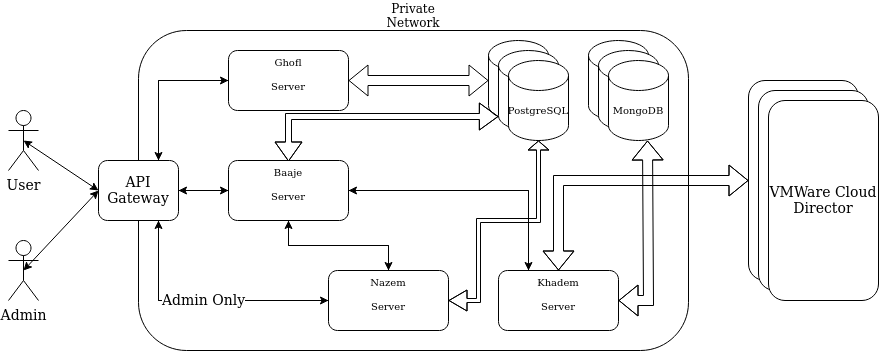
\includegraphics[scale=0.5]{figures/30bird-arch.png}
	\caption{معماری کلی سامانه}
	\label{fig:30bird-arch}
\end{figure}


\clearpage
\section{میکروسرویس‌ها}
کل سامانه از چهار میکروسرویس تشکیل شده: قفل، ناظم، خادم و باجه. هر میکروسرویس، مخصوص رسیدگی به امور بخشی از سامانه است. این میکروسرویس‌ها در قالب معماری کد تک مخزنه\LTRfootnote{Mono Repo} پیاده‌سازی شده‌اند و دارای اشتراک‌های زیادی در کد‌های پایه هستند.

\subsection{جزئیات فنی مشترک}
در این بخش قصد داریم که این موارد مشترک را مطرح کنیم و سپس به بررسی جزئیات اختصاصی هر سرویس بپردازیم.

این موارد شامل:

\begin{itemize}
	\item خدمت‌گزار وب
	\item برنامه‌ی تحت خط‌‌فرمان
	\item مدیریت تنظیمات
	\item تعامل با پایگاه داده و مدیریت مدل‌ها
	\item ساختار کد
\end{itemize}
می‌شود که در ادامه‌ی این بخش به شرح جزئیات هر‌یک می‌پردازیم.


اجرای یک خدمت‌گزار وب\LTRfootnote{Web Server} توسط چهارچوب \lr{Echo} در زبان \lr{Go} انجام می‌شود. نحوه عملکرد این چهارچوب به این شکل است که در ابتدا قوانین مربوط به مسیریاب\LTRfootnote{Router} تنظیم می‌شود، سپس برای هر مقصد\LTRfootnote{Endpoint}، یک رسیدگی کننده\LTRfootnote{Handler} تعریف می‌کنیم. به عنوان مثال برای عملیات ورود کاربر به سامانه، برای مسیر \lr{/api/login} یک رسیدگی کننده تعریف می‌کنیم که عملیات لازم جهت ورود کاربر را اجرا می‌کند. این عملیات در این مثال شامل چک کردن ورودی درخواست، اتصال به پایگاه داده، چک کردن صحت اطلاعات فرستاده شده و ارسال یک کلید ورود برای کاربر است که همگی در قالب یک تابع به عنوان رسیدگی کننده‌ی این مقصد تعریف می‌شوند. همچنین در تمامی خدمت‌گزار‌های این سامانه، کاربران بایستی هویت خود را از طریق سربرگ‌های اجباری از پیش تعیین شده مشخص کنند و یک احراز هویت با کلید ثابت انجام دهند. این امر جهت بالا بردن امنیت دوچندان سامانه تعبیه شده‌است.
در ساختار کد این پروژه، ثبت این مقصدها به همراه توابع رسیدگی کننده در بسته \lr{api/http/handler} انجام می‌شود. جهت ثبت یک بسته جدید فقط کافیست که مشخصات مقصد و تابع رسیدگی کننده در فایلی داخل این بسته نوشته شود و با تابع \lr{RegisterEndpoints} مقصد مورد نظر داخل مسیریاب \lr{Echo} ثبت شود.

معماری کلی عملکرد \lr{Echo} در شکل\ref{fig:echo-workflow} و پوشه‌بندی موارد گفته شده در شکل\ref{fig:echo-folder-router} و \ref{fig:echo-folder-handler} توضیح داده شده‌است.

\begin{figure}
	\centering
	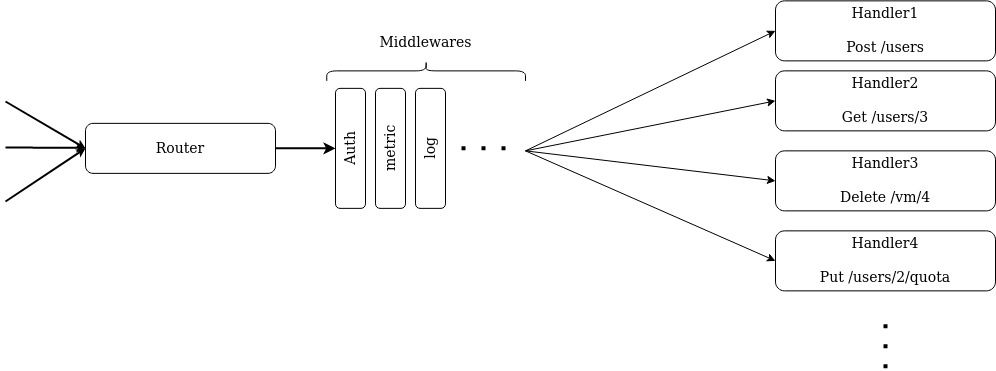
\includegraphics[scale=0.45]{figures/echo-workflow.jpeg}
	\caption{عملکرد چهارچوب \lr{Echo}}
	\label{fig:echo-workflow}
\end{figure}

\begin{figure}
	\vspace{1cm}
	\centering
	\begin{minipage}[b]{0.5\textwidth}
		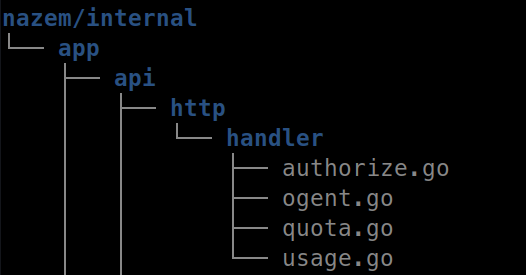
\includegraphics[width=\textwidth]{figures/echo-handler-dir.png}
		\caption{پوشه‌بندی توابع رسیدگی‌کننده \lr{Echo}}
		\label{fig:echo-folder-handler}
	\end{minipage}
	\hfill
	\begin{minipage}[b]{0.4\textwidth}
		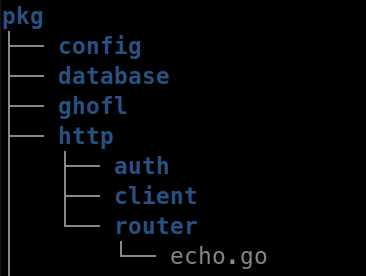
\includegraphics[width=\textwidth]{figures/echo-router-dir.png}
		\caption{پوشه‌بندی مسیریاب \lr{Echo}}
		\label{fig:echo-folder-router}
	\end{minipage}
	
\end{figure}


ایجاد برنامه‌های تحت خط‌فرمان\LTRfootnote{Command Line Application} توسط چهارچوب \lr{Cobra} پیاده‌سازی شده‌است. این چهارچوب به برنامه‌نویسان این اختیار ‌را می‌دهد که برای برنامه‌های خود یک رابط خط فرمان\LTRfootnote{Command Line Interface} ایجاد کنند. با این کار، برنامه‌نویس می‌تواند با کد‌های نوشته شده برای پروژه، چندین فرمان قابل اجرا ایجاد کند. مزیت این‌کار در سناریو‌هایی که برنامه‌ی‌ نوشته شده نیاز به اجرای چند فرمان مختلف به طور همزمان در پس‌زمینه داشته باشد مشخص می‌شود.

برنامه ‌های خط فرمان طبق پوشه‌بندی شکل\ref{fig:cobra-dir} در پروژه‌ها قرار گرفته‌اند.

\begin{figure}
	\vspace{1cm}
	\centering
	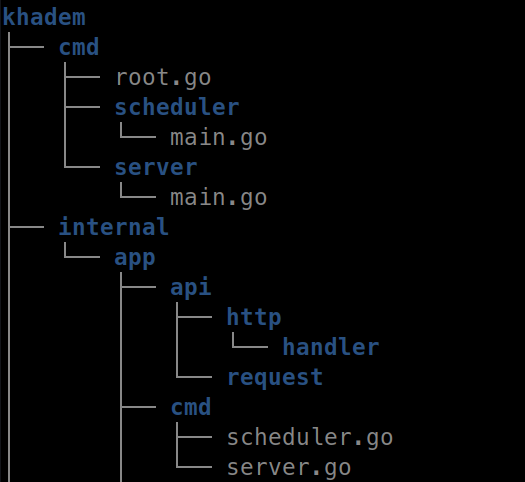
\includegraphics[scale=0.45]{figures/cobra-dir.png}
	\caption{ساختار پوشه‌بندی برنامه‌های خط فرمان در پروژه خادم}
	\label{fig:cobra-dir}
\end{figure}

مدیریت تنظیمات برنامه توسط چهارچوب \lr{Viper} انجام می‌شود. این چهارچوب، به کاربران این اجازه را می‌دهد که تنظیمات را در هر‌یک از ساختارهای معروف \lr{JSON}، \lr{YAML} و یا \lr{TOML} بنویسد و با قراردادن آن در یکی از آدرس‌های پیشفرض تنظیمات، آن‌ها را بر روی برنامه اعمال کند. ساختار انتخابی ما برای تنظیمات به صورت پیش‌فرض، ساختار \lr{YAML} است که در یک فایل هم‌اسم پروژه، در پوشه ریشه پروژه قرار گرفته.

تنظیمات برنامه می‌تواند در یکی از آدرس‌های زیر باشد.
\begin{enumerate}
	\item \lr{./<appname>.yaml}
	\item \lr{/etc/<appname>/<appname>.yaml}
	\item \lr{~/.config/<appname>.yaml}
\end{enumerate}


تعامل و ارتباطات با پایگاه داده در اپلیکیشن‌ها با دو چهارچوب \lr{gorm} و \lr{ent} انجام می‌شود. مزیت چهارچوب \lr{gorm}، سادگی عملکرد و گستردگی پشتیبانی و جامعه متن‌باز آن است. هر دو چهارچوب به عنوان یک \lr{ORM}\LTRfootnote{Object-Relation Mapping} تعامل با پایگاه داده را بسیار ساده‌تر می‌کنند. به گونه‌ای که برای ارتباط با پایگاه‌داده به هیچ‌عنوان دغدغه‌ی نحوه تعریف روابط و ذخیره‌سازی اطلاعات را نداریم و فقط با مدل‌های تعریف شده‌ی داخل برنامه تعامل برقرار می‌کنیم. در کد این پروژه، ارتباطات با پایگاه داده جهت دریافت و ثبت اطلاعات در یک لایه‌ی کاملا مجزا با استفاده از الگوی شیئ دسترسی داده\LTRfootnote{Data Access Object} پیاده‌سازی شده است. این الگوی طراحی به نویسندگان کد این امکان را می‌‌دهد، که توابع و نیازمندی‌های دسترسی به داده ذخیره‌شده را در یک لایه‌ی کاملا جداگانه تعریف کنند و لایه‌های دخل و تصرف داده را در کنار این لایه توسعه دهند\cite{oracle_dao}.

با توجه به این‌که چهارچوب \lr{ent} توسط تولید کد رابط‌های مورد نیاز جهت تعامل با پایگاه داده را فراهم می‌کند، تمامی ریسک‌ها و خطر‌های امنیتی مربوط به پایگاه داده به علت \lr{Type Safe} بودن این رابط قابل کنترل می‌شود. این مورد یکی از مزیت‌های بسیار بزرگ استفاده از این چهارچوب است.

تمامی کد‌های مربوط به تعامل با پایگاه داده مطابق شکل\ref{fig:ent}، در پوشه \lr{ent} قرار گرفته‌است. جزئیات مهم این پوشه‌بندی به شرح زیر می‌باشد.

\begin{itemize}
	\item \lr{\textbf{schema}}: این پوشه شامل تعاریف ساختار مدل‌ها در پایگاه داده است.
	\item \lr{\textbf{entc.go}}: در این فایل، قوانین تولید و تفسیر \lr{API} تعامل با پایگاه داده قرار داده شده است.
	\item \lr{\textbf{generate.go}}: این فایل، نحوه تولید فایل‌های خودکار تولید‌شده را مشخص می‌کند.
	\item \lr{\textbf{openapi.json}}: این فایل، ساختار و مشخصات \lr{API} تولید‌شده را بر اساس استاندارد \lr{OpenAPI} مشخص می‌کند.
\end{itemize}

\begin{figure}
	\vspace{1cm}
	\centering
	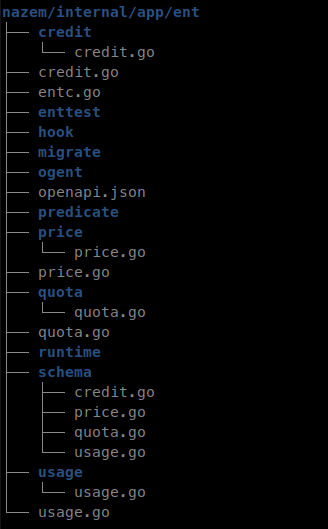
\includegraphics[scale=0.45]{figures/ent.png}
	\caption{ساختار پوشه‌بندی چهارچوب \lr{ent}}
	\label{fig:ent}
\end{figure}

با توجه به استفاده از الگوی تک‌مخزنه در نگهداری کد‌های پروژه، تا حد ممکن کد‌ها و منابع مشترک پروژه در پوشه \lr{pkg} نگهداری می‌شود. 

ساختار این پوشه در شکل\ref{fig:pkg-dir} مشخص شده، توضیحات پوشه‌های موجود در این ساختار به شرح زیر می‌باشد.
\begin{itemize}
	\item \lr{\textbf{config}}: نحوه خوانده شدن تنظیمات و قوانین مربوط به پردازش تنظیمات که بین پروژه‌ها مشترک است در فایل‌های این پوشه نوشته شده‌است.
	\item \lr{\textbf{database}}: کد‌های مربوط به نحوه اتصال به پایگاه داده و مکانیزم‌های تلاش مجدد در فایل‌های این پوشه قرار داده شده، در صورت نیاز به پشتیبانی از پایگاه داده جدید، فقط کافیست نحوه اتصال به پایگاه داده را داخل این پوشه مشخص کنیم.
	\item \lr{\textbf{http}}: میان‌افزارهای مشترک، تنظیمات مسیریاب اولیه برنامه، به همراه فایل‌های کاربر\LTRfootnote{Client}‌های برنامه‌ها در این پوشه تعبیه شده‌است.
	\item \lr{\textbf{log}}: تنظیمات مربوط به راه‌اندازی ثبت کننده وقایع در این پوشه انجام می‌شود.
	\item \lr{\textbf{model}}: مدل‌های مشترک نظیر ماشین مجازی یا تنظیمات آن در هر یک داخل فایلی داخل این پوشه قرار داده می‌شود.
\end{itemize}

\begin{figure}
	\vspace{1cm}
	\centering
	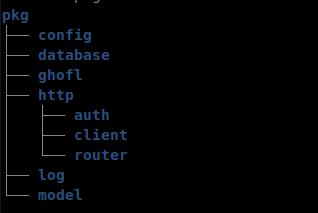
\includegraphics[scale=0.55]{figures/pkg-dir.png}
	\caption{ساختار پوشه‌بندی \lr{pkg}}
	\label{fig:pkg-dir}
\end{figure}

\subsection{قفل}
میکروسرویس مخصوص احراز‌ هویت و تعیین سطح دسترسی در این سامانه، قفل نام دارد. دلیل نام‌گذاری این میکروسرویس به این اسم، شباهت عملکرد قفل و این سامانه است که هر دو وظیفه کنترل دسترسی به منابع پشت قفل را دارند.

\begin{figure}
	\vspace{1cm}
	\centering
	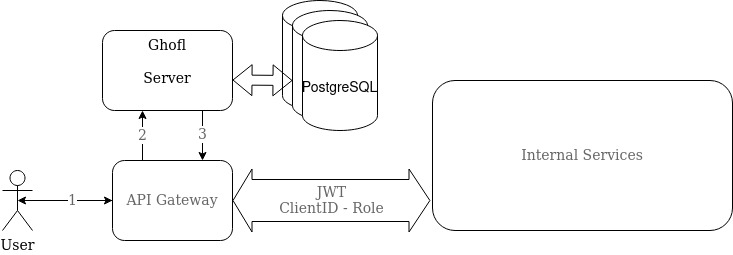
\includegraphics[scale=0.5]{figures/30bird-ghofl.jpg}
	\caption{عملکرد سرویس قفل}
	\label{fig:30bird-ghofl}
\end{figure}

در شکل\ref{fig:30bird-ghofl}، کاربرد سرویس قفل در سامانه مشخص شده‌است. \textbf{تمامی درخواست‌های ورودی} به سامانه در ابتدا به سرویس قفل فرستاده می‌شوند و احراز هویت آن‌ها انجام می‌شود. این درخواست‌ها یا مانند درخواست ورود و ثبت‌نام ماهیت احراز هویت دارند و یا سایر درخواست‌های کاربری و مدیریتی هستند. دسته اول درخواست‌ها مستقیما به قفل فرستاده می‌شوند. دسته دوم درخواست‌ها نیز هنگام رسیدن به دروازه ‌ورود، ابتدا به قفل فرستاده می‌شوند که سرایند احراز هویت \lr{JWT}\LTRfootnote{JSON Web Token} آنها ارزیابی شود. پس از این ارزیابی، در صورت موفقیت آمیز‌بودن. درخواست به سرویس‌های بالادستی فرستاده شده و درصورت ورود ناموفق کاربر با خطا مواجه خواهد شد.


پوشه بندی این پروژه در شکل\ref{fig:30bird-ghofl-dir} مشخص شده است. 
در این پوشه‌بندی، پوشه \lr{auth} مربوط به منطق‌های لازم جهت پیاده سازی احراز هویت است. 

\begin{figure}
	\vspace{1cm}
	\centering
	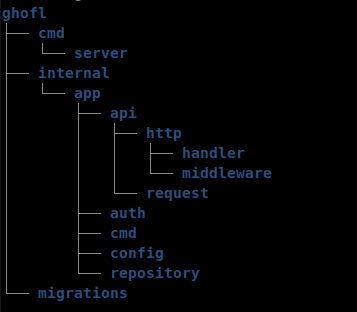
\includegraphics[scale=0.5]{figures/ghofl-dir.png}
	\caption{پوشه بندی سرویس قفل}
	\label{fig:30bird-ghofl-dir}
\end{figure}

\subsection{ناظم}
میکروسرویس ناظم وظیفه نظارت و مدیریت امور مالی و گزارشات مصرف کاربران را برعهده دارد. این میکروسرویس یکی از کلیدی‌ترین سرویس‌های سامانه است که در تعامل زیاد با پایگاه داده است. معماری کلی این سرویس در شکل\ref{fig:30bird-nazem} مشخص شده‌است.

ناظم در \textbf{تعامل با باجه} در جایگاه یک اعتبارسنج\LTRfootnote{Validator} درخواست عمل می‌کند. به این صورت که تمامی درخواست‌های مربوط به دخل و تصرف در منابع باید ابتدا از این سامانه تاییدیه بگیرند. گرفتن این تاییدیه به معنی اعتبار کافی و نبودن محدودیت بر روی کاربر برای منابع درخواستی است. هرگونه ایراد و خطا در این سرویس منجر توقف عملکرد کل سامانه است که این امر یک موضوع پیش‌بینی شده و قابل قبول است. کد‌های مربوط به این اعتبار سنجی داخل بسته \lr{validation} قرار گرفته و برای توسعه و تغییر این قوانین باید این بسته دچار تغییر شود.

در تعامل با ‌دروازه‌ی ورود، درخواست‌های مدیر سامانه جهت تغییر محدودیت‌های کاربران یا گزارش گیری از وضعیت آنان را دریافت می‌کند و پاسخ مناسب را با توجه به اطلاعات ثبت شده در پایگاه داده می‌دهد.

این سرویس برای درخواست‌های دریافتی از سرویس خادم، گزارش مصرف منابع را برای منابع دریافت می‌کند و با توجه به قوانین و قیمت گذاری‌های ثبت‌شده، اعتبار کاربر را تحت تاثیر قرار می‌دهد.

\begin{figure}
	\vspace{1cm}
	\centering
	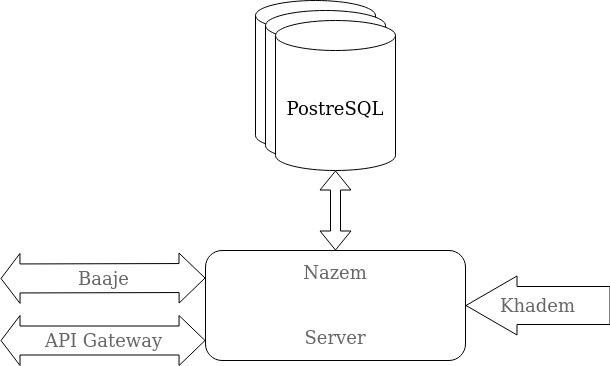
\includegraphics[scale=0.7]{figures/30bird-nazem.jpg}
	\caption{عملکرد سرویس ناظم}
	\label{fig:30bird-nazem}
\end{figure}

پوشه‌بندی بسته ها در این پروژه در شکل\ref{fig:30bird-nazem-dir} مشخص شده‌است. در این پوشه‌بندی، بسته‌ی \lr{billing} شامل منطق‌های لازم جهت صحت‌سنجی درخواست‌های تغییر منابع می‌باشد که داخل توابع رسیدگی‌کننده به همین‌نام استفاده شده

بسته‌ی مهم دیگر، بسته \lr{usage} می‌باشد که قوانین مربوط به نحوه ثبت و بروزرسانی مصرف منابع کاربر در آن تعریف و پیاده‌سازی شده‌است.

\begin{figure}
	\vspace{1cm}
	\centering
	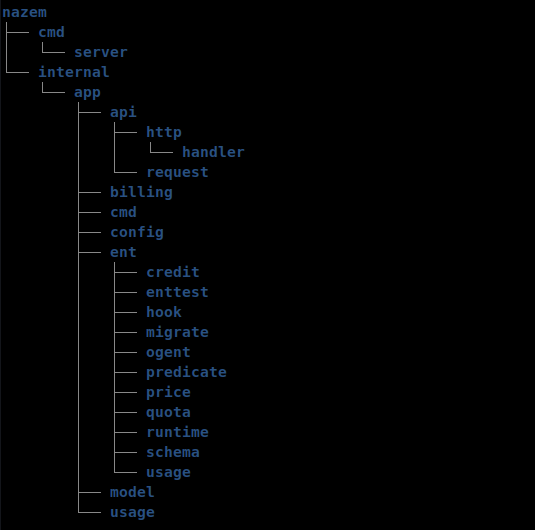
\includegraphics[scale=0.8]{figures/nazem-dir.png}
	\caption{پوشه بندی سرویس ناظم}
	\label{fig:30bird-nazem-dir}
\end{figure}


\subsection{باجه}
این سرویس دروازه ارتباطی کاربران عادی سامانه است. تمامی درخواست‌ها و عملیات ممکن برای کاربر در این برنامه قرار گرفته. معماری این برنامه در شکل\ref{fig:30bird-baaje} مشخص شده است. همانطور که در تصویر مشخص شده، این سرویس مستقیما از طریق ‌دروازه‌ی ورود با کاربران در ارتباط است و برای انجام امور مربوط به کاربران با سرویس‌های خادم و ناظم به صورت داخلی در ارتباط است.


این سرویس اطلاعات مربوط به منابع تعریف شده برای کاربر را داخل پایگاه داده ذخیره کرده و در پردازش درخواست‌ها از این اطلاعات استفاده می‌کند. منابع تعریف شده داخل پایگاه داده شده داخل پیوست این گزارش موجود است.

در مواجه با درخواست‌های مربوط به تغییر منابع مانند ساخت یا ویرایش ماشین مجازی، ابتدا اعتبارسنجی درخواست از طریق سرویس ناظم انجام می‌شود و در صورت موفقیت‌آمیز بودن این اعتبارسنجی، درخواست جهت اجرا به سرویس خادم ارسال می‌شود. پس از رسیدن جواب از سمت سرویس خادم، بسته به خروجی سرویس خادم، نتیجه درخواست کاربر داخل پایگاه داده ذخیره می‌شود.

این قابلیت‌ها توسط بسته‌بندی‌ای که در شکل\ref{fig:30bird-baaje-dir} مشخص شده پیاده‌سازی شده‌اند. اکثر کد‌های این سرویس داخل بسته \lr{handler} قرار‌دارد که با بسته‌های کاربر بقیه سرویس‌ها، با آن‌ها به تعامل می‌پردازد.
بسته دیگری که مختص این پروژه می‌باشد، بسته \lr{validate} است که یک رابط برای سرویس ناظم است، در صورت تقسیم شدن سرویس ناظم  و یا تغییر منطق صحت‌سنجی درخواست‌ها فقط باید محتوی این بسته را تغییر داد و توابع رسیدگی کننده بدون تغییر خواهندبود.
\begin{figure}
	\centering
	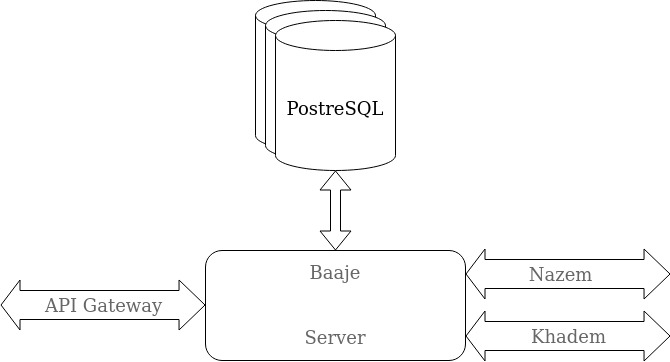
\includegraphics[scale=0.5]{figures/30bird-baaje.jpg}
	\caption{عملکرد سرویس باجه}
	\label{fig:30bird-baaje}
\end{figure}

\begin{figure}
	\vspace{1cm}
	\centering
	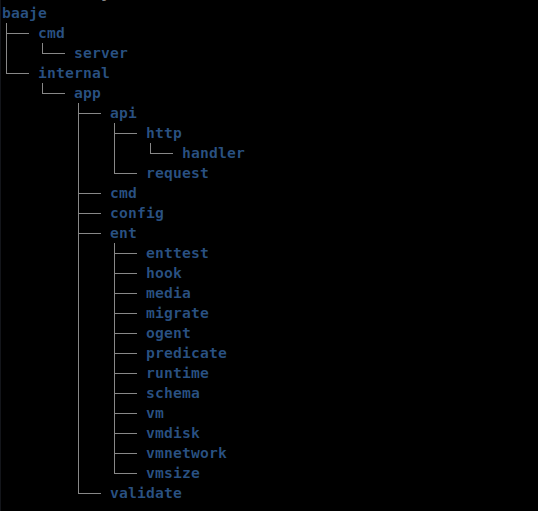
\includegraphics[scale=0.7]{figures/baaje-dir.png}
	\caption{پوشه بندی سرویس باجه}
	\label{fig:30bird-baaje-dir}
\end{figure}


\begin{figure}
	\vspace{1cm}
	\centering
	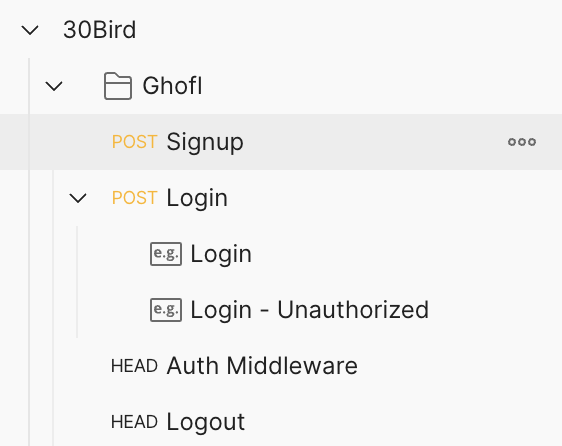
\includegraphics[scale=0.7]{figures/ghofl-api.png}
	\caption{لیست \lr{Endpoint}های سرویس قفل}
	\label{fig:ghofl-api}
\end{figure}


\begin{figure}
	\vspace{1cm}
	\centering
	\begin{minipage}[b]{0.45\textwidth}
		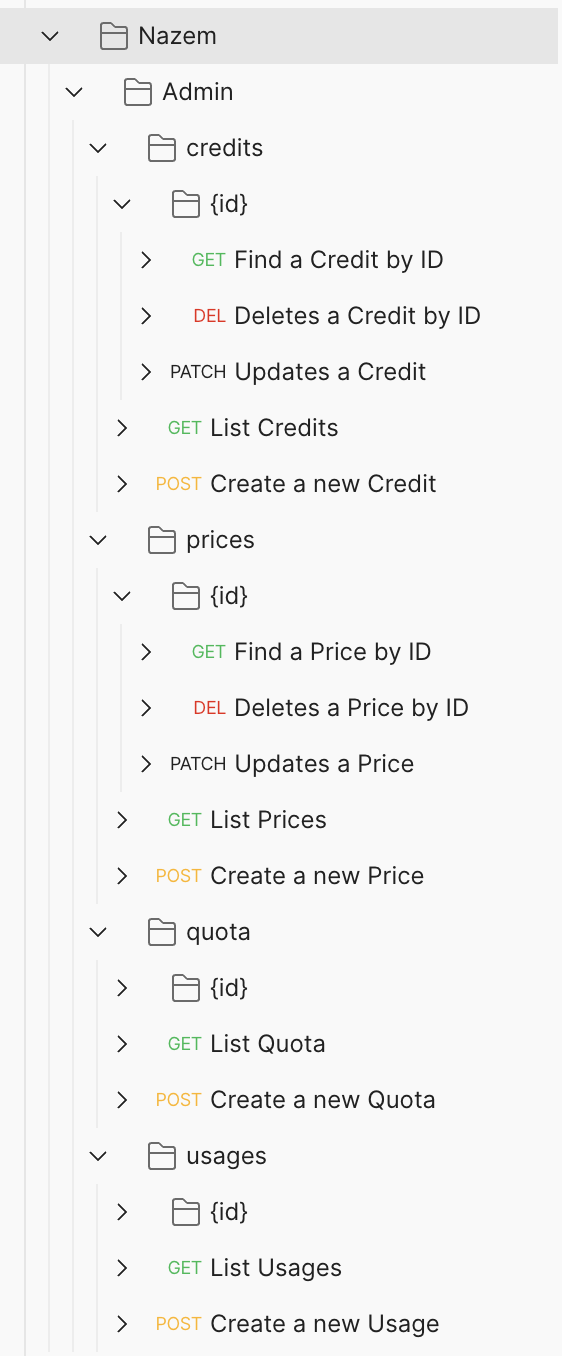
\includegraphics[width=\textwidth]{figures/nazem-api.png}
		\caption{لیست \lr{Endpoint}های سرویس ناظم}
		\label{fig:nazem-api}
	\end{minipage}
	\hfill
	\begin{minipage}[b]{0.45\textwidth}
		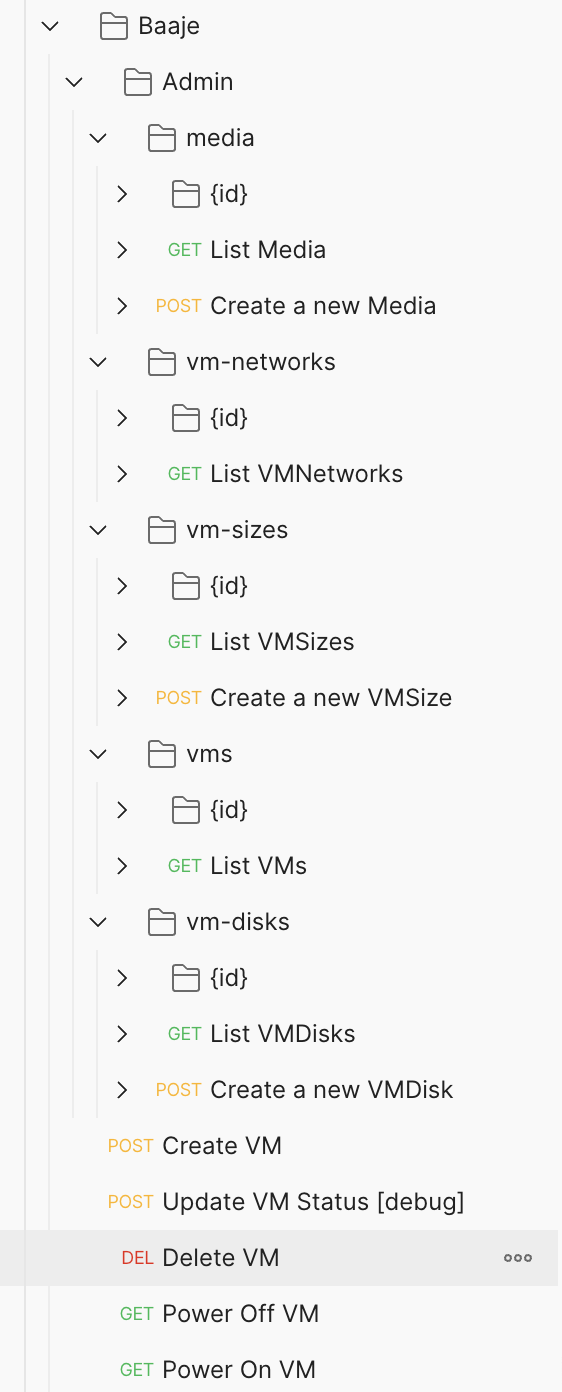
\includegraphics[width=\textwidth]{figures/baaje-api.png}
\caption{لیست \lr{Endpoint}های سرویس باجه}
\label{fig:baaje-api}
	\end{minipage}
	
\end{figure}


\clearpage
\subsection{خادم}
همانطور که قبلا گفته شد، سامانه برای ارائه خدمات \lr{IaaS} نیازمند تعامل با یک ارائه دهنده زیرساخت است. این ارائه دهنده در سامانه‌ما \lr{VMWare Cloud Director} است، میکروسرویس مسئول جهت تعامل با این برنامه خادم است. معماری خادم از دو قسمت اصلی تشکیل شده است. \textbf{خدمت‌گزار} و \textbf{زمان‌بند}\LTRfootnote{Scheduler} دو بخش تشکیل دهنده این سرویس می‌باشند که کاملا مستقل و جداگانه اجرا می‌شوند. وظیفه خدمت‌گزار دریافت دستورات از سرویس باجه و سپس تفسیر و اجرای آن‌‌ها است. معماری کلی این پروژه در شکل \ref{fig:30bird-khadem}مشخص شده است.

بسته‌بندی پروژه در شکل\ref{fig:30bird-khadem-dir} مشخص شده‌است.

\begin{figure}
	\vspace{1cm}
	\centering
	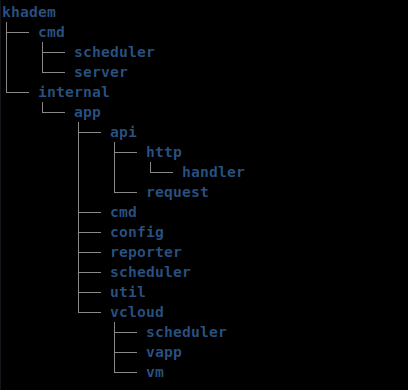
\includegraphics[scale=0.7]{figures/khadem-dir.png}
	\caption{پوشه بندی سرویس خادم}
	\label{fig:30bird-khadem-dir}
\end{figure}

پایه کد این پروژه به طور کلی در بسته \lr{vcloud} قرار داده شده‌است. این بسته شامل تمامی عملیات قابل اجرا بر روی \lr{cloud director} است. در صورت نیاز به تکمیل و یا توسعه خدمات بایستی دستورات و توابع این بسته را تغییر داد. داخل این بسته از بسته توسعه نرم‌افزار (\lr{SDK}\LTRfootnote{Software Development Kit}) رسمی \lr{VMWare Cloud Director} استفاده شده‌است. البته برای کاربرد‌های خاص و عملیات تخصصی دقیق، ممکن است که نیاز به تعامل مستقیم با \lr{API} داشته باشیم. ولی برای خدمات فعلی سامانه، تمامی امکانات مورد نیاز داخل \lr{SDK} موجود است.

منطق‌های مربوط به نظارت کننده منابع که وظیفه گزارش مصرف منابع‌ را بر عهده دارد، در بسته \lr{scheduler} قرار دارد. در این بسته یک اجراشونده کار در پس زمینه فراخوانی شده و عملیات دریافت وضعیت منابع و ارسال این اطلاعات به سرویس ناظم را انجام می‌دهد.

پوشه مهم دیگر داخل پروژه، پوشه \lr{reporter} است. این پوشه وظیفه اطلاع‌رسانی وضعیت نهایی درخواست‌های ارسال شده به خادم  به سرویس‌های بالادستی را برعهده دارد. از نمونه‌ی این اطلاع‌رسانی‌ها، می‌توان به گزارش وضعیت ماشین مجازی ساخته‌شده و اطلاعات شبکه‌ای آن مانند آدرس \lr{IP} آن اشاره کرد که بایستی به سرویس باجه فرستاده‌شود که وضعیت ماشین مجازی در پایگاه داده را بروزرسانی کند.

همچنین یک ثبت کننده وقایع داخل این سرویس تعبیه شده که تمامی درخواست‌های ارسالی به سرویس‌ بالا‌دستی را در یک پایگاه داده غیر رابطه‌ای ذخیره کند. این کار برای نظارت بیشتر و بازیابی از حادثه\LTRfootnote{Incident Recovery} احتمالی بسیار مفید است.

\begin{figure}
	\centering
	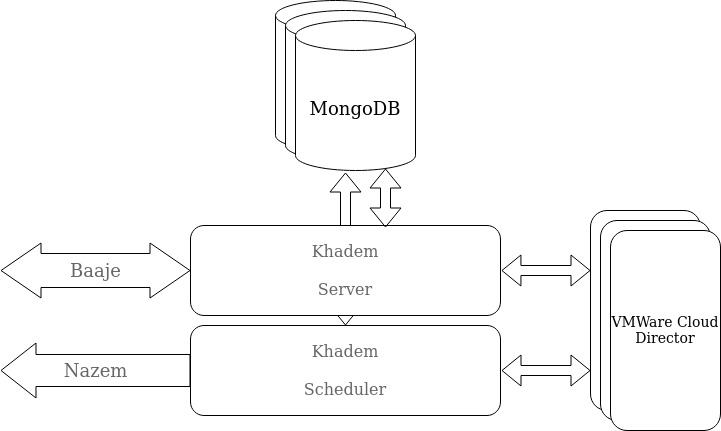
\includegraphics[scale=0.5]{figures/30bird-khadem.jpeg}
	\caption{عملکرد سرویس خادم}
	\label{fig:30bird-khadem}
\end{figure}

برنامه \textbf{زمان‌بند} در پس‌زمینه به صورت مستقل اجرا شده و در فواصل زمانی مشخص وضعیت منابع تعریف شده داخل \lr{Cloud Director} را رصد کرده و گزارش وضعیت را به سرویس ناظم جهت رسیدگی به امور مالی و نظارتی ارسال می‌کند. یک محدودیت مهم این سرویس، تک نسخه ای بودن آن در زمان اجرا است. برای قابلیت چند نسخه‌ای بودن این برنامه، بایستی یک مکانیزم و الگوریتم هماهنگی میان عناصر درحال اجرا پیاده‌سازی کنیم که منابع سیستم در هر لحظه تنها \textbf{توسط فقط یک نسخه} رصد و گزارش شود. پیاده‌سازی این موضوع با کمک امکانات کوبرنتیز امکان پذیر است ولی بخاطر پیچیدگی‌هایی که این پیاده‌سازی به همراه دارد در این پروژه از این‌کار صرف نظر شده‌است.

برنامه خدمت‌گزار در پس‌زمینه اجرا می‌شود و منتظر دستورات از سمت باجه می‌شود. پس از رسیدن دستورات، بسته به نوع دستور، توابع و پیاده‌سازی‌های موجود در بسته \lr{vcloud} در برنامه اجرا می‌شود. با این کار، دستورات قابل فهم توسط \lr{cloud director} ارسال شده و نتیجه به صورت برخط و یا غیر برخط به کاربر گزارش می‌شود.


\section{‌دروازه‌ی ورود رابط}
پیاده‌سازی ‌دروازه‌ی ورود رابط در این سامانه با استفاده از ابزار قدرتمند و پایدار \lr{nginx} صورت گرفته. \lr{nginx} یک خدمت‌گزار وب نوشته شده با زبان \lr{C} است که توانایی مدیریت تعداد بسیار زیادی از درخواست‌ها در لحظه را دارد. برای استفاده از این ‌دروازه‌ی ورود باید قوانین مربوط به مسیریابی را در فرمت مخصوص بنویسیم. از آنجایی که مقیاس کردن این گزینه به صورت افقی سخت انجام می‌شود (باید قوانین مربوط به \lr{DNS} و کاربران را تغییر دهیم.) بایستی منابع و ظرفیت‌های این برنامه‌ را زیاد‌تر از سایر قسمت‌های دیگر در نظر بگیریم.

\section{خطایابی}
عملکرد مورد انتظار رابط‌های برنامه‌نویسی برنامه در فایل‌های \lr{Open API Specification} نوشته‌شده، می‌توان این فایل‌ها را با استفاده از ابزار \lr{Swagger} بررسی کرد. در صورتی که سامانه نتیجه‌ای غیر از نتیجه انتظار برگرداند. خطایابی با استفاده از کد وضعیت برگردانده شده به همراه پیام\LTRfootnote{Message} پاسخ می‌تواند انجام شود. در صورت نیاز به اطلاعات بیشتر، برنامه‌ها خطا‌های رخ‌داده را داخل \lr{Std Error} محیط اجرایی چاپ می‌کنند. در صورت اجرا در قالب بسته‌های داکر، چک کردن این خطا‌ها می‌تواند با دستور \lr{docker logs} انجام شود. با توجه به سطوح مختلف اطلاع رسانی خطا، تنظیمات چاپ رخداد‌ها را می‌شود داخل فایل \lr{config} تغییر داد. درجات مختلف چاپ جزئیات در لیست زیر نوشته شده‌است. در این لیست اولین عضو به معنی کمترین جزئیات و آخرین عضو به معنی بیشترین جزئیات است.

\begin{enumerate}
	\item \lr{panic}
	\item \lr{fatal}
	\item \lr{error}
	\item \lr{warning}
	\item \lr{info}
	\item \lr{debug}
\end{enumerate}


\section{نتیجه گیری}
در این فصل به تشریح قسمت‌های مختلف برنامه و جزئیات پیاده‌سازی آن‌ها پرداخته شد. سامانه ما از چهار میکروسرویس که هریک وظیفه مخصوص به خود را دارد تشکیل شد. این میکروسرویس‌ها که در قالب بسته‌های داکر اجرا شدند با رابط‌های \lr{REST} به یکدیگر متصل هستند. همه این میکروسرویس‌ها در پشت یک ‌دروازه‌ی ورود قرار گرفته و راه ارتباطی با شبکه خصوصی سامانه تنها این ‌دروازه‌ی ورود است. اولین میکروسرویس درگیر با درخواست‌های کاربران، \textbf{قفل} هست که وظیفه احراز هویت تمامی درخواست‌های ورودی به ‌دروازه‌ی ورود را دارد. میکروسرویس بعدی، \textbf{باجه} است که تمامی عملیات کاربران در آن تعریف شد. این میکروسرویس برای صحت سنجی درخواست‌های کاربران با میکروسرویس \textbf{ناظم} در ارتباط است و برای انجام این درخواست‌ها با میکروسرویس \textbf{خادم} ارتباط برقرار می‌کند.

